\section{Toky v sítích}
\begin{t_definition}
  Síť je pětice $(V, E, s, t, c)$, kde $G=(V,E)$ je orientovaný graf, $c:E\rightarrow\mathbb{R}$ je zobrazení přiřazující hranám v $G$ jejich kapacitu. Vrcholy $s,t\in V$ jsou zvláštní vrcholy v $G$, které nazýváme jako zdroj a stok.
\end{t_definition}

\begin{t_definition}
  Ohodnocení hran orientovaného grafu $(V,E)$ je funkce $f:E\rightarrow\mathbb{R}$. Pro každé ohodnocení definujeme:
  \begin{enumerate}
    \item \textit{Co do vrcholu přiteče:} $f^+(v)=\sum_{e=(\cdot,v)} f(e)$, kde $v\in V$,
    \item \textit{Co z vrcholu odteče:} $f^-(v)=\sum_{e=(v,\cdot)} f(e)$, kde $v\in V$,
    \item \textit{Přebytek:} $f^\Delta(v)=f^+(v)-f^-(v)$.
  \end{enumerate}
\end{t_definition}

\begin{t_observation}
  Je-li $(V, E, s, t, c)$ síť, potom je funkce $c$ ohodnocením hran grafu $(V,E)$.
\end{t_observation}

\begin{t_definition}
  Tok v síti $(V, E, s, t, c)$ je ohodnocení $f$ takové, že platí:
  \begin{enumerate}
    \item
    \textit{Tok je v mezích kapacity každé hrany.}\\
    $\forall e\in E : 0\leq f(e) \leq c(e)$
    
    \item
    \textit{Kirchhoffův zákon: vstupní tok vrcholu je roven výstupnímu toku.}\\
    $\forall v\in V, v\neq s, t : f^\Delta(v)=0$
  \end{enumerate}
\end{t_definition}

\begin{t_definition}
  Velikost toku $f$ v síti $(V, E, s, t, c)$ definujeme $|f|=-f^\Delta(s)$.
\end{t_definition}

\begin{t_remark}
  Hlavní úlohou teorie toků je hledání tzv. maximálního toku, tedy toku s maximální velikostí. Pojďme si ukázat algoritmus, který tento problém z části řeší.
\end{t_remark}

\begin{t_definition}
  Hladový algoritmus využíváme k nalezení maximálního toku $f$ v síti $(V, E, s, t, c)$. Není ale optimálním algoritmem pro tento druh úlohy!
  
  \begin{algorithm}
    \caption{Hladový algoritmus}
    \begin{algorithmic}[1]
      \State $f\gets$ \textit{nulový tok}
      \Repeat
      \State Najdeme cestu $P$ z vrcholu $s$ do $t$.
      \State Vylepšíme tok $f$ na hranách cesty $P$ na maximální možný.
      \Until{všechny cesty v $G$ jsou nasyceny}
    \end{algorithmic}
  \end{algorithm}
\end{t_definition}

\begin{t_definition}
  Pro srozumitelnost zápisu zavedeme následující označení pro množiny vrcholů $X\subseteq V$ a $Y\subseteq V$ v síti $(V, E, s, t, c)$:
  \begin{enumerate}
    \item $X^+=\{(u,v)\in E\mid u\notin X, v\in X\}$ \textit{množina hran vedoucích do vrcholů v $X$},
    \item $X^-=\{(u,v)\in E\mid u\in X, v\notin X\}$ \textit{množina hran vedoucích z vrcholů v $X$},
    \item $E(X,Y)=\{(u,v)\in E\mid u\in X, v\in Y\}$ \textit{množina hran vedoucích z vrcholů $X$ do $Y$}.
  \end{enumerate}
\end{t_definition}

\begin{t_definition}
  Tokový řez v síti $(V, E, s, t, c)$ je množina $C\subset V$ taková, že $s\in C$, $t\notin C$.
\end{t_definition}

\begin{t_definition}
  Kapacitu řezu $C$ v síti $(V, E, s, t, c)$ definujeme $|C|=\sum_{e\in C^-} c(e)$.
\end{t_definition}

\begin{t_remark}
  Jak uvidíme v dalších větách, maximální tok má úzkou souvislost s tzv. minimálním řezem, tedy řezem, jehož kapacita je minimální.
\end{t_remark}

\begin{t_fact}
  V každé síti existuje maximální tok a minimální řez.
\end{t_fact}

\begin{t_definition}
  Řez $C$ v síti $(V, E, s, t, c)$ je elementární, pokud existuje množina vrcholů $A\subseteq V$ taková, že $s\in A,t\notin A$ a $C=E(A,V\setminus A)$.
\end{t_definition}

\begin{t_lemma}[o elementárním řezu]
  V síti $(V, E, s, t, c)$ každý řez $C$ obsahuje jako podmnožinu elementární řez $A$.
\end{t_lemma}

\begin{t_proof}
  Vezmeme libovolný řez $C$, pozorujeme, že nám síť rozdělí na dvě množiny vrcholů spojené s vrcholy $s$ a $t$. Označme tu z nich, která obsahuje vrchol $s$ jako množinu $A^\prime$. V této množině najdeme všechny vrcholy dosažitelné cestou z vrcholu $s$, označme je jako $A$. Zkonstruujeme nový řez $D=E(A,V\setminus A)$ – nahlédneme, že je elementární.
\end{t_proof}

\begin{t_corollary}
  Řez je elementární, pokud je minimální v inkluzi.
\end{t_corollary}

\begin{t_definition}
  Pro tok $f$ a řez $C$ v síti $(V, E, s, t, c)$ definujeme:
  \begin{enumerate}
    \item \textit{Co do řezu přiteče:} $f^+(C)=\sum_{e\in C^+} f(e)$,
    \item \textit{Co z řezu odteče:} $f^-(C)=\sum_{e\in C^-} f(e)$,
    \item \textit{Přebytek:} $f^\Delta(C)=f^+(C)-f^-(C)$.
  \end{enumerate}
\end{t_definition}

\begin{t_lemma}[omezení toku řezem]
  Pro každý tok $f$ a řez $C$ v síti $(V, E, s, t, c)$ platí: $|f|=-f^\Delta(C)\leq|C|$.
\end{t_lemma}

\begin{t_proof}
  Nejprve dokážeme rovnost $|f|=-f^\Delta(s)=-f^\Delta(C)$. To uděláme s pomocí matematické indukce. Nahlédneme, že každý řez můžeme sestrojit postupným přidáváním vrcholů do triviálního řezu $\{s\}$. Z definice vyplývá, že $|f|=-f^\Delta(s)=-f^\Delta(\{s\})$. Počáteční podmínka tedy platí. Nyní ukážeme, že při přidání vrcholu do řezu se $f^\Delta$ nezmění.
  
  Mějme řez $C$, pro který platí $-f^\Delta(C)=-f^\Delta(s)$, a vrchol $x\in V, x\neq s, t$ takový, že $x\notin C$. Vytvoříme řez $C^\prime=C\cup x$ a chceme ukázat, že $-f^\Delta(C)=-f^\Delta(C^\prime)$. Uvažme všechny hrany vrcholu $x$, každou hranu $e$ můžeme zařadit do jedné z kategorií:
  \begin{enumerate}
    \item Hrana $e$ vede z $x$ do vrcholu v $C$. Potom její přidání k řezu $C$ sníží $f^-(C)$.
    \item Hrana $e$ vede z vrcholu v $C$ do $x$. Potom její přidání k řezu $C$ sníží $f^+(C)$.
    \item Hrana $e$ vede z $x$ do vrcholu mimo $C$. Potom její přidání k řezu $C$ zvýší $f^+(C)$.
    \item Hrana $e$ vede z vrcholu mimo $C$ do $x$. Potom její přidání k řezu $C$ zvýší $f^-(C)$.
  \end{enumerate}
  
  Z Kirchhoffova zákona přitom víme, že $f^\Delta(x)=0$, z čehož vyplývá $f^+(x)=f^-(x)$. Když uvedené kategorie seskupíme podle orientace hran na $x$, zjistíme, že hrany v kategoriích 1 a 3 přispívají do $f^+(x)$ a hrany v kategoriích 2 a 4 přispívají do $f^-(x)$.
  
  Souhrnný příspěvek všech hran z kategorie 1 do $f^+(x)$ můžeme vyjádřit jako snížení $f^-(C)$, analogicky souhrnný příspěvek hran z kategorie 3 vyjádříme jako zvýšení $f^+(C)$. Pokud takto vyjádříme i souhrnný příspěvek do $f^-(x)$ ze zbylých dvou kategorií, získáme z původní rovnosti $f^+(x)=f^-(x)$ následující výraz.
  \begin{align*}
    \overbrace{(f^-(C)-f^-(C^\prime))}^{\textrm{kategorie 1}}+\overbrace{(f^+(C^\prime)-f^+(C))}^{\textrm{kategorie 3}}&=
    \overbrace{(f^+(C)-f^+(C^\prime))}^{\textrm{kategorie 2}}+\overbrace{(f^-(C^\prime)-f^-(C))}^{\textrm{kategorie 4}}\\
    2f^+(C^\prime)-2f^-(C^\prime)&=2f^+(C)-2f^-(C)\\
    2f^\Delta(C^\prime)&=2f^\Delta(C)
  \end{align*}
  
  Jednoduchými ekvivalentními úpravami tento výraz převedeme na rovnost, kterou jsme chtěli dokázat. Z toho plyne, že pro každý řez $C$ umíme nejprve sestrojíme posloupnost řezů $C_1, C_2\dots C_k$ takovou, že $C_1=\{s\}$, $C_k=C$ a pro všechna $i$ platí $|C_{i+1}\setminus C_i|=1$. V této posloupnosti musí navíc platit $f^\Delta(C_i)=f^\Delta(C_{i+1})$. Není už složité nahlédnout, že $|f|=-f^\Delta(s)=-f^\Delta(C_1)=-f^\Delta(C_2)=\dots=-f^\Delta(C_k)=-f^\Delta(C)$. Tím je důkaz první rovnosti dokončen.
  
  V druhé části důkazu vyjdeme z definice:
  \begin{align*}
    -f^\Delta(C)=f^-(C)-f^+(C)\leq f^-(C)
    =\sum_{e\in C^-} f(e)\leq \sum_{e\in C^-} c(e)=|C|
  \end{align*}
\end{t_proof}

\begin{t_theorem}[Fordova-Fulkersonova, minimaxová]
  V každé síti je velikost maximálního toku rovna kapacitě minimálního řezu.
\end{t_theorem}

\begin{t_proof}
  Z předchozího lemmatu plyne, že velikost maximálního toku je nejvýše rovna kapacitě minimálního řezu. Opačná nerovnost vyplyne z Fordova-Fulkersonova algoritmu.
\end{t_proof}

\begin{t_definition}
  Buď síť $(V, E, s, t, c)$, $f$ tok, $e$ a $e^\prime$ dvojice opačných hran. Potom je rezerva hrany $e$ definována:
  \begin{align*}
    r(e)=c(e)-f(e)+f(e^\prime)
  \end{align*}
\end{t_definition}

\begin{t_remark}
  Pro jednoduchost v této definici předpokládáme, že ke každé hraně existuje i hrana opačná. Pro hrany, které tuto vlastnost nesplňují, rezervu dodefinujeme, jako by opačná hrana měla nulový tok:
  \begin{align*}
    r(e)=c(e)-f(e)
  \end{align*}
\end{t_remark}

\begin{t_definition}
  Buď síť $(V, E, s, t, c)$ a $f$ tok. Zlepšující cesta je orientovaná cesta na $(V,E)$ taková, že všechny její hrany mají nenulovou rezervu.
\end{t_definition}

\begin{t_definition}
  Vylepšením hladového algoritmu je Fordův-Fulkersonův algoritmus.
  
  \begin{algorithm}
    \caption{Fordův-Fulkersonův algoritmus}
    \begin{algorithmic}[1]
      \State $f\gets$ \textit{nulový tok}
      \While{existuje zlepšující cesta $P$ z $s$ do $t$}
      \State $\varepsilon\gets\min_{e\in P} r(e)$
      \Comment $\varepsilon$ je největší možné zlepšení $P$
      \ForAll{$e\in P$}
        \If{hrana $e$ je ve směru z $s$ do $t$}
          \State $f(e)\gets f(e)+\varepsilon$
        \Else
          \State $f(e)\gets f(e)-\varepsilon$
        \EndIf
      \EndFor
      \EndWhile
    \end{algorithmic}
  \end{algorithm}
\end{t_definition}

\begin{t_claim}
  V síti s racionálními kapacitami Fordův-Fulkersonův algoritmus terminuje.
\end{t_claim}

\begin{t_proof}
  Nejdříve se omezíme jen na síť s celočíselnými kapacitami. Pozorujeme, že na takové síti algoritmus doběhne, protože v každém kroku stoupne velikost toku o $\varepsilon\geq 1$, což může nastat pouze konečněkrát. V síti s racionálními kapacitami můžeme všechny kapacity vynásobit jejich společným jmenovatelem a získáme tak síť s celočíselnými kapacitami, čímž jsme problém převedli na předchozí případ. 
\end{t_proof}

\begin{t_remark}
  Pokud je alespoň jedna kapacita iracionální, Fordův-Fulkersonův algoritmus obecně terminovat nemusí.
\end{t_remark}

\begin{t_remark}
  Časová složitost Fordova-Fulkersonova algoritmu závisí na volbě zlepšujících cest. Pokud budeme hledat cesty prohledáváním do šířky (Edmonds, Karp), algoritmus poběží v čase $O(m^2n)$. Pokud budou navíc kapacity jednotkové, snadno nahlédneme, že stačí $O(mn)$.
\end{t_remark}

\begin{t_claim}
  Pokud Fordův-Fulkersonův algoritmus terminuje, najde maximální tok.
\end{t_claim}

\begin{t_proof}
  Uvažme situaci po zastavení algoritmu. Funkce $f$ je určitě tok, protože jím byla po celou dobu běhu algoritmu. Prozkoumejme množinu $C$ vrcholů, do nichž po zastavení algoritmu vede zlepšující cesta ze zdroje. Jistě $s\in C$ a $t\notin C$, takže tato množina je řez. Navíc pro každou hranu $e\in C^-$ musí být $f(e)=c(e)$ a pro každou $e^\prime\in C^+$ je $f(e^\prime)=0$, jinak by rezerva hrany byla nenulová a existovala by další zlepšující cesta. Takže $f^-(C)=|C|$ a $f^+(C)=0$, čili $|f|=|C|$.
  
  Našli jsme tedy k toku, který algoritmus vydal, řez stejné velikosti, a proto, jak už víme, je tok maximální a řez minimální. Tím jsme také dokázali Fordovu-Fulkersonovu větu a existenci maximálního toku.
\end{t_proof}

\begin{t_corollary}
  Síť s celočíselnými kapacitami má maximální tok, který je celočíselný.
\end{t_corollary}

\begin{t_proof}
  Z předchozího důkazu vyplývá, že algoritmus nikdy nevytváří z celých čísel necelá.
\end{t_proof}

\begin{t_exercise}
  \item Najděte maximální tok z $v_1$ do $v_7$.
  \begin{figure}[!htbp]
    \centering
    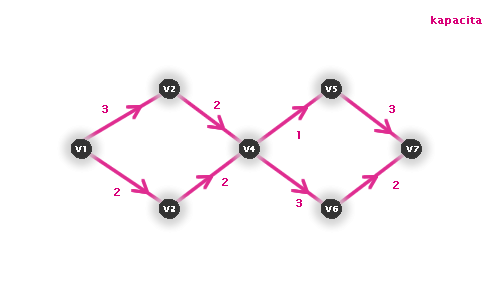
\includegraphics[width=0.7\textwidth]{img/net1.png}
  \end{figure}
  
  \item Najděte maximální tok z $v_1$ do $v_6$.
  \begin{figure}[!htbp]
    \centering
    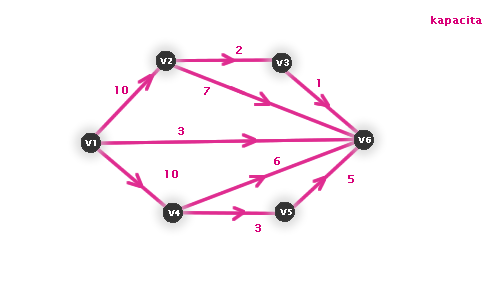
\includegraphics[width=0.7\textwidth]{img/net2.png}
  \end{figure}
  
  \item Najděte maximální tok z $v_1$ do $v_6$.
  \begin{figure}[!htbp]
    \centering
    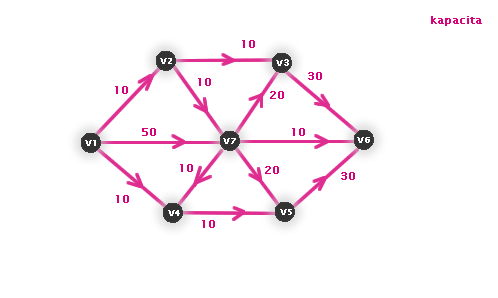
\includegraphics[width=0.7\textwidth]{img/net3.png}
  \end{figure}
  
  \item Najděte maximální tok z $v_1$ do $v_5$.
  \begin{figure}[!htbp]
    \centering
    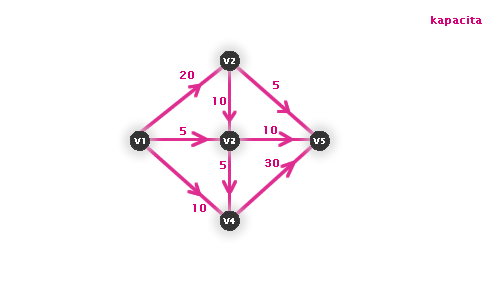
\includegraphics[width=0.7\textwidth]{img/net4.png}
  \end{figure}
  
  \item Najděte maximální tok z $v_1$ do $v_8$.
  \begin{figure}[!htbp]
    \centering
    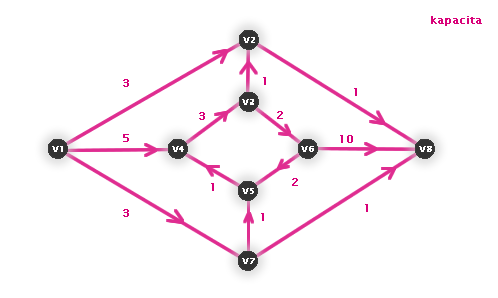
\includegraphics[width=0.7\textwidth]{img/net5.png}
  \end{figure}
\end{t_exercise}
